\documentclass{article}
\usepackage{fullpage}

%load needed packages
\usepackage{graphicx}
\usepackage{array}
\usepackage{booktabs}
\usepackage[utf8]{inputenc}
\usepackage[T1]{fontenc}
\usepackage{url}
\usepackage[spanish]{babel} % Paquete para el idioma español
\usepackage{float}  % Necesario para [H]
\usepackage{listings}
\usepackage{xcolor}

\definecolor{codegreen}{HTML}{5AB2FF}
\definecolor{morado}{HTML}{AD88C6}
\definecolor{BG}{HTML}{EEEEEE}
\definecolor{azul}{HTML}{4D869C}
\definecolor{sqlblue}{HTML}{FF8C00} % Color para las palabras clave SQL

% Estilo para DDL
\lstdefinestyle{ddlstyle}{
	language=SQL,
	backgroundcolor=\color{BG},
	commentstyle=\color{codegreen},
	basicstyle=\ttfamily\small,
	keywordstyle=\color{azul},
	stringstyle=\color{morado},
	showstringspaces=false,
	breaklines=true,
	frame=shadowbox,
	numbers=left,
	numberstyle=\tiny\color{gray},
	captionpos=b,
}

% Estilo para SQL
\lstdefinestyle{sqlstyle}{
	language=SQL,
	backgroundcolor=\color{BG},
	commentstyle=\color{codegreen},
	basicstyle=\ttfamily\small,
	keywordstyle=\color{sqlblue}, % Color diferente para palabras clave SQL
	stringstyle=\color{morado},
	showstringspaces=false,
	breaklines=true,
	frame=shadowbox,
	numbers=left,
	numberstyle=\tiny\color{gray},
	captionpos=b,
}

\begin{document}
	
	
	
	% Portada
	\begin{titlepage}
		\centering
		\vspace*{3cm}
		
		% Título destacado
		{\Huge \textbf{Estracción, Transformación y Carga de datos en Almacén de Gasto en Medicamento}\\[0.5cm]}
		
		% Espacio y logotipo (si lo tienes, por ejemplo el logo de tu universidad)
		\vspace{2cm}
		
\includegraphics[width=0.3\textwidth]{images/uma_logo.jpg}\\[1cm]
		
		% Nombre del autor
		{\LARGE \textbf{Alejandro Silva Rodríguez}\\[0.5cm]}
		{\LARGE \textbf{Marta Cuevas Rodríguez}\\[0.5cm]}
		{\large \textit{Almacenes De Datos}\\
			Universidad de Málaga\\
		}
		
		\vfill
		
		% Fecha en la parte inferior de la página
		{\large Diciembre 2024}
	\end{titlepage}
	
	% indice
	\tableofcontents
	
	\newpage
	\section{Introducción}
	\label{sec:introduccion}
	
	En el contexto hospitalario actual, el monitoreo y la gestión eficiente de los recursos es una necesidad apremiante, especialmente en unidades como la de Cuidados Intensivos (UCI), donde la administración de medicamentos representa una parte sustancial de los costos. A nivel mundial, el incremento en el costo de los medicamentos y la presión financiera sobre los sistemas de salud han impulsado la búsqueda de soluciones que optimicen el uso de los recursos en entornos críticos. Sin embargo, muchas instituciones hospitalarias carecen de herramientas analíticas específicas para monitorizar y analizar de manera detallada el gasto en fármacos, lo que limita la capacidad de identificar patrones de consumo y optimizar la asignación de presupuestos.\\
	
	En el informe anterior se detalló el diseño e implementación de un almacén de datos diseñado para analizar el gasto en medicamentos en pacientes ingresados en la UCI en hospitales de EE.UU a partir de la base de datos proporcionada por el MIT \cite{eicu_crd}. Para abordar este desafío, el proceso de extracción, transformación y carga (ETL) se convierte en un componente clave, ya que permite integrar datos de diferentes fuentes, transformarlos en un formato homogéneo y almacenarlos en el almacén de datos. Este enfoque no solo facilita el análisis eficiente del gasto en medicamentos, sino que también garantiza la calidad y coherencia de los datos utilizados para la toma de decisiones.
	
	\section{Objetivos}
	\label{sec:objetivos}
	
	El objetivo principal de este trabajo es implementar procesos de extracción, transformación y carga (ETL) para alimentar de manera eficiente dos almacenes de datos: el almacén NorthwindDW y un almacén diseñado para analizar el gasto en medicamentos en unidades de cuidados intensivos (UCI). Este propósito se concreta en los siguientes objetivos específicos:
	
	\begin{itemize}
		\item Diseñar y ejecutar un proceso ETL completo para el almacén de datos NorthwindDW, utilizando herramientas y técnicas previamente estudiadas, con el fin de consolidar conocimientos y garantizar la correcta carga de todas sus tablas.
		\item Corregir el diseño del almacén de datos, de manera que facilite los procesos ETL.
		\item Implementar un proceso ETL personalizado para un almacén de datos orientado al análisis del gasto en medicamentos en las UCI.
		
	\end{itemize}
	
	\section{Almacén de Datos de NorthWind}
	
	El objetivo de esta parte del proyecto consiste en construir un almacén de datos (\texttt{NorthwindDW}) a partir de la base de datos \texttt{Northwind}. Para ello, se desarrolló un proceso de extracción, transformación y carga (ETL) que permite mover los datos desde la base de datos origen hacia el almacén, adaptándolos a su nueva estructura.
	
	\subsection{Extracción, Transformación y Carga de Datos}
	
	El flujo ETL diseñado se compone de múltiples tareas que se ejecutan de manera secuencial y/o paralela. Estas tareas incluyen la carga de diferentes dimensiones como \texttt{Employee}, \texttt{Category}, \texttt{Product}, entre otras, así como tablas relacionadas con jerarquías geográficas como \texttt{Continent}, \texttt{Country}, \texttt{State}, y \texttt{City}. Cada tarea se asegura de transformar los datos según las necesidades del almacén y garantizar su integridad y consistencia.
	\\
	
	En la Figura \ref{fig:NorthWind}, se presenta el flujo de control completo con todas las tareas ejecutadas satisfactoriamente. Este diagrama refleja el correcto funcionamiento del proceso ETL y el éxito en la carga de los datos.
	
	\begin{figure}[H]
		\begin{center} 
			\includegraphics[width=0.65\textwidth]{images/cargaNorthwind.png} % Cambia 1 a 0.5 o el valor deseado
			\caption{Carga completa del almacén NorthwindDW}
			\label{fig:NorthWind}
		\end{center}
	\end{figure}
	
	\subsection{Dificultades encontradas}
	Durante la implementación del proceso ETL (Extract, Transform, Load), se encontraron ciertas dificultades. Una de ellas ocurrió durante la carga de la tabla \texttt{Employee}. Al intentar insertar datos, surgió el siguiente error (Listing \ref{lst:error}) relacionado con restricciones de claves foráneas:
	
	\begin{lstlisting}[style=ddlstyle, label=lst:error,caption=Error al llenar empleado]
	[Empleado DW [68]] Error: An exception has occurred during 
	data insertion, the message returned from the provider is: 
	Se termino la instruccion. Instruccion INSERT en conflicto 
	con la restriccion FOREIGN KEY SAME TABLE 'FK_Employee_Employee'. 
	El conflicto ha aparecido en la base de datos 'NorthwindDW', 
	tabla 'dbo.Employee', column 'EmployeeKey'.
	\end{lstlisting}
	
	Este problema se debía a que la tabla \texttt{Employee} contenía una clave foránea que referenciaba a sí misma, lo cual generaba conflictos al insertar los datos en un orden incorrecto. Para resolverlo, se deshabilitaron temporalmente las restricciones de claves foráneas antes de la carga de datos mediante el comando Listing \ref{lst:Deshabilitar}.
	
	
	\begin{lstlisting}[style=ddlstyle, label=lst:Deshabilitar,caption=Deshabilitar restricciones en empleado]
	EXEC sp_MSForEachTable 'ALTER TABLE ? NOCHECK CONSTRAINT ALL';
	\end{lstlisting}
	
	Una vez finalizada la carga de datos, se volvieron a habilitar las restricciones para asegurar la integridad referencial del almacén con el siguiente comando Listing \ref{lst:Habilitar}
	
	
	\begin{lstlisting}[style=ddlstyle, label=lst:Habilitar,caption=Habilitar restricciones en empleado]
	EXEC sp_MSForEachTable 'ALTER TABLE ? WITH CHECK CHECK CONSTRAINT ALL';
	\end{lstlisting}
	
	Gracias a esta solución, el proceso de carga se completó exitosamente. 
	
	\section{Almacén de Datos de Gasto de Medicamento en UCI}
	
	\subsection{Rediseño del Almacén}
	
	Antes de proceder con el llenado del almacén, se realizó un rediseño significativo de su estructura para optimizar su funcionamiento y facilitar la integración con la base de datos de origen. 
	\begin{figure}[H]
		\begin{center} 
			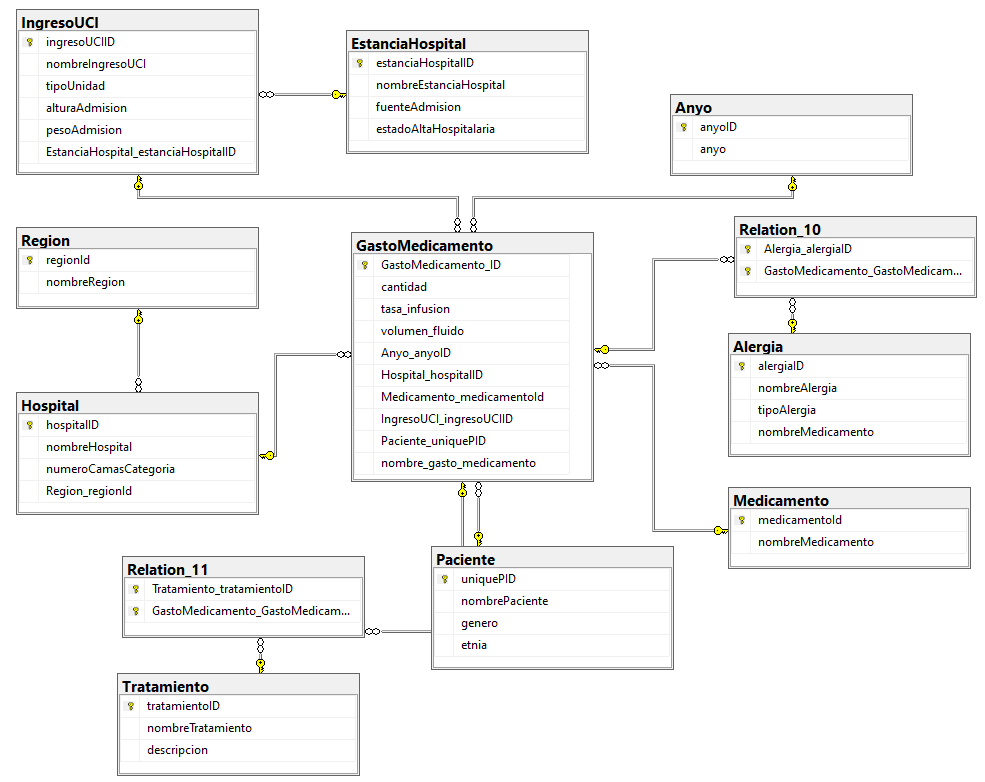
\includegraphics[width=0.65\textwidth]{images/nuevo_diseno.png} % Cambia 1 a 0.5 o el valor deseado
			\caption{Rediseño del almacén para gastos en medicamentos}
			\label{fig:nuevo_diseño}
		\end{center}
	\end{figure}
	Como se puede observar en la Figura \ref{fig:nuevo_diseño}, este rediseño incluye varios cambios clave:
	
	\begin{itemize}
		\item \textbf{Autogeneración de identificadores (IDs):} En el nuevo diseño, los identificadores principales de las tablas ahora son generados automáticamente por el sistema, en lugar de depender de los valores provenientes de la base de datos de origen. Esto asegura consistencia y evita problemas de duplicados.
		
		\item \textbf{Preservación de IDs originales como atributos:} Los identificadores originales de la base de datos de origen se han mantenido, pero ahora figuran como atributos adicionales en las clases correspondientes. Esto permite rastrear fácilmente el origen de los datos y establecer vínculos con sistemas externos cuando sea necesario. Cabe puntualizar que esto ha sido solo añadido en las tablas donde sería imposible buscar sin tener ese identificador.
		
		\item \textbf{Adición de nuevos atributos:} Se han incorporado más atributos en algunas tablas para enriquecer la información almacenada. Por ejemplo:
		\begin{itemize}
			\item En la tabla \texttt{Paciente}, se han añadido atributos como el género y la etnia.
			\item La tabla \texttt{EstanciaHospital} incluye ahora información sobre la fuente de admisión y el estado al alta hospitalaria.
			\item La tabla \texttt{GastoMedicamento} incluye atributos como el volumen de fluido y el tipo de infusión.
		\end{itemize}
	\end{itemize}
	
	Estos cambios no solo mejoran la estructura y la claridad del diseño del almacén, sino que también amplían su capacidad para almacenar información detallada, facilitando futuros análisis y consultas complejas.
	
	
	\subsection{Creación de un Nuevo Proyecto en SQL Server Management Studio}
	
	A continuación, se describe el proceso para crear un nuevo proyecto en SQL Server Management Studio (SSMS), paso a paso:
	
	\paragraph{Paso 1: Abrir SQL Server Management Studio}  
	Abre SQL Server Management Studio desde el menú de inicio de tu sistema operativo. Si no lo tienes instalado, puedes descargarlo desde el sitio oficial de Microsoft.
	
	\paragraph{Paso 2: Iniciar un Nuevo Proyecto}  
	Sigue los pasos a continuación para crear un nuevo proyecto en SSMS:
	\begin{enumerate}
		\item En el menú principal de SSMS, haz clic en \textbf{Archivo} (\textit{File}).
		\item Selecciona \textbf{Nuevo Proyecto} (\textit{New Project}).
		\item En la ventana emergente, selecciona el tipo de proyecto llamado \textbf{Proyecto de Base de Datos} (\textit{Database Project}).
		\item Asigna un nombre a tu proyecto en el campo \textbf{Nombre del Proyecto} (\textit{Project Name}), como por ejemplo: \texttt{etl\_uciDW}.
		\item Elige una ubicación para guardar tu proyecto en el campo \textbf{Ubicación} (\textit{Location}).
		\item Haz clic en \textbf{Aceptar} (\textit{OK}) para crear el proyecto.
	\end{enumerate}
	
	\paragraph{Paso 3: Configurar Conexión a la Base de Datos}  
	Una vez creado el proyecto:
	\begin{enumerate}
		\item En la barra de herramientas de SSMS, haz clic en \textbf{Ver} (\textit{View}) y selecciona \textbf{Explorador de Objetos} (\textit{Object Explorer}).
		\item En el panel de \textit{Object Explorer}, haz clic derecho sobre \textbf{Conexiones de Servidor} (\textit{Server Connections}) y selecciona \textbf{Conectar} (\textit{Connect}).
		\item Introduce los detalles de conexión a tu servidor SQL, como:
		\begin{itemize}
			\item Nombre del servidor (\textit{Server Name}): Por ejemplo, \texttt{localhost} o el nombre de tu servidor.
			\item Tipo de autenticación (\textit{Authentication}): Selecciona \texttt{Windows Authentication} o \texttt{SQL Server Authentication} según corresponda.
		\end{itemize}
		\item Haz clic en \textbf{Conectar} (\textit{Connect}) para enlazar el proyecto con la base de datos deseada.
	\end{enumerate}
	
	
	\subsection{Extracción, Transformación y Carga de Datos}
	
	\subsection{Flujo general de carga del almacén}
	Antes de pasar explicando en detalle la carga de cada tabla, observamos en la Figura \ref{fig:flujo_general} el flujo general de la carga. Por un lado se cargan las tablas más simples (Medicamento, Paciente y Anyo) que se mapean directamente en el almacén, por otro lado se cargan las dimensiones con dos niveles (Estancia Hosiptal-Ingreso UCI y Hospital-Región) que necesitarán que sean cargadas de forma secuencial. Después se añadirá el hecho y por último las relaciones M:N con el hecho. Para garantizar que no hay problemas con duplicados borraremos el almacén al principio del flujo en cada ejecución.
	\begin{figure}[H]
		\centering
		\label{fig:flujo_general}
		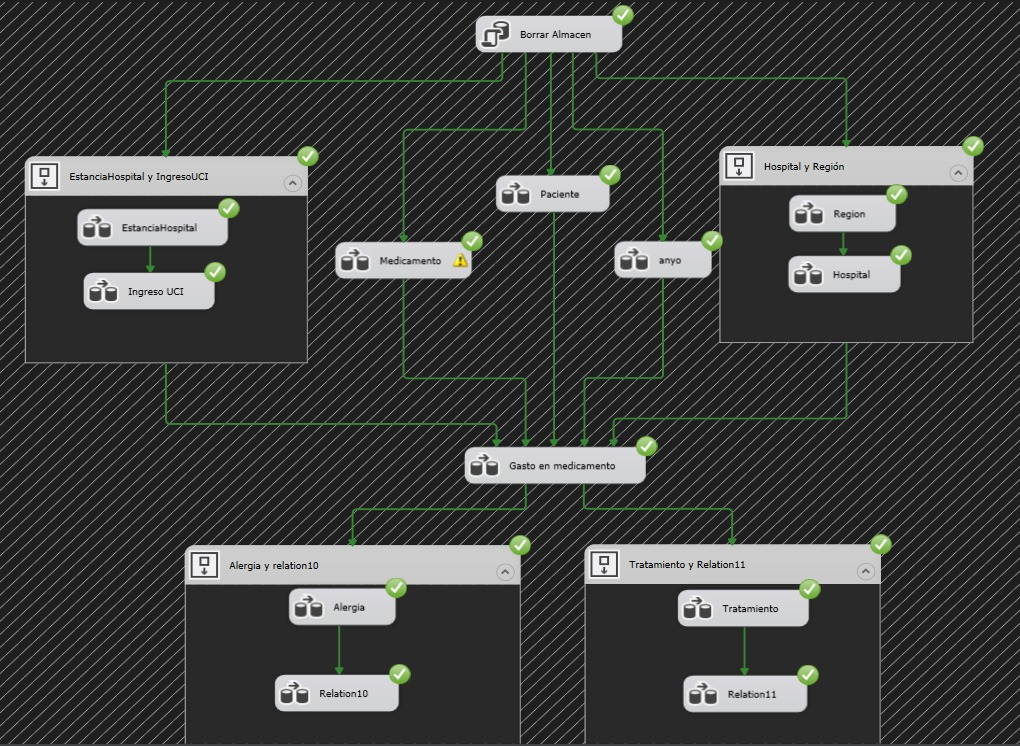
\includegraphics[width=\linewidth]{./images/completados/flujo_completo_uci.jpeg}
		\caption{Carga completa del almacén UCI de gasto en medicamentos}
	\end{figure}
	\subsubsection{Borrado del Almacén}
	
	Para realizar el borrado completo del almacén de datos, es necesario crear un procedimiento almacenado en SQL Server Management Studio (SSMS). Esto se lleva a cabo en el almacén de datos, accediendo a la sección \texttt{Programmability} y creando un nuevo \texttt{Stored Procedure}. \\
	
	El procedimiento debe incluir las instrucciones necesarias para eliminar los datos de las tablas en el orden correcto, comenzando por las tablas que tienen dependencias externas (o relaciones con otras tablas) y finalizando con aquellas más internas (las que no tienen dependencias hacia otras tablas). Esto asegura que las restricciones de claves foráneas no causen errores durante el proceso de eliminación.
	
	\begin{lstlisting}[style=ddlstyle, label=fig:borradoAlmacen,caption=Borrado del Almacen de UCI]
		USE UCIDW;
		GO
		SET ANSI_NULLS ON;
		GO
		SET QUOTED_IDENTIFIER ON;
		GO
		CREATE OR ALTER PROCEDURE BorrarAlmacen	
		AS
		BEGIN
		BEGIN TRY
		-- Iniciar transaccion
		BEGIN TRANSACTION;
		-- Eliminar datos de las tablas
		DELETE FROM Relation_10;
		DELETE FROM Relation_11;
		DELETE FROM GastoMedicamento;
		DELETE FROM Medicamento;
		DELETE FROM Alergia;
		DELETE FROM Anyo;
		DELETE FROM Tratamiento;
		DELETE FROM Hospital;
		DELETE FROM Region;
		DELETE FROM IngresoUCI;
		DELETE FROM EstanciaHospital;
		DELETE FROM Paciente;
		-- Reiniciar los valores de identidad
		DBCC CHECKIDENT ('Medicamento', RESEED, 0);
		DBCC CHECKIDENT ('Alergia', RESEED, 0);
		DBCC CHECKIDENT ('Tratamiento', RESEED, 0);
		DBCC CHECKIDENT ('Region', RESEED, 0);
		DBCC CHECKIDENT ('Hospital', RESEED, 0);
		DBCC CHECKIDENT ('EstanciaHospital', RESEED, 0);
		DBCC CHECKIDENT ('IngresoUCI', RESEED, 0);
		DBCC CHECKIDENT ('Paciente', RESEED, 0);
		DBCC CHECKIDENT ('GastoMedicamento', RESEED, 0);
		-- Confirmar transaccion
		COMMIT TRANSACTION;
		END TRY
		BEGIN CATCH
		-- Deshacer transaccion si ocurre un error
		IF @@TRANCOUNT > 0
		ROLLBACK TRANSACTION;
		-- Rethrow del error para depuracion
		THROW;
		END CATCH;
		END;
		GO
	\end{lstlisting}
	
	
	En el \texttt{Listing \ref{fig:borradoAlmacen}}, se describe el contenido del procedimiento almacenado \texttt{BorrarAlmacen}, que realiza las siguientes operaciones clave:
	
	\begin{enumerate}
		\item \textbf{Inicio de una transacción:} Se utiliza \texttt{BEGIN TRANSACTION} para garantizar que todas las operaciones de eliminación se realicen de forma atómica. En caso de que ocurra un error, la transacción puede revertirse completamente mediante \texttt{ROLLBACK TRANSACTION}.
		
		\item \textbf{Eliminación de datos:} Los datos se eliminan de todas las tablas, siguiendo el orden correcto:
		\begin{itemize}
			\item Se empieza eliminando las relaciones secundarias (\texttt{Relation\_10} y \texttt{Relation\_11}).
			\item Posteriormente, se eliminan las tablas principales como \texttt{GastoMedicamento}, \texttt{Medicamento}, \texttt{Alergia}, \texttt{Anyo}, \texttt{Tratamiento}, \texttt{Hospital}, \texttt{Region}, \texttt{IngresoUCI}, \texttt{EstanciaHospital} y \texttt{Paciente}.
		\end{itemize}
		
		\item \textbf{Reinicio de valores de identidad:} Después de eliminar los datos, se reinician los valores de identidad en las tablas afectadas usando el comando \texttt{DBCC CHECKIDENT}. Esto asegura que los identificadores autogenerados comiencen desde cero para futuras inserciones.
		
		\item \textbf{Confirmación de la transacción:} Una vez completadas todas las eliminaciones y reinicios, la transacción se confirma mediante \texttt{COMMIT TRANSACTION}.
		
		\item \textbf{Gestión de errores:} En caso de un error, el bloque \texttt{CATCH} revierte la transacción para preservar la integridad del almacén de datos y re-lanza la excepción con el comando \texttt{THROW}, facilitando la depuración.
	\end{enumerate}
	
	Este procedimiento asegura que el almacén de datos esté completamente vacío y listo para ser llenado nuevamente, mientras se mantiene la consistencia y se manejan posibles errores durante el proceso.
	
	\subsection{Añadiendo el Procedimiento de Borrado al Proyecto}
	
	Para integrar el procedimiento \texttt{BorrarAlmacen} en el flujo de trabajo del proyecto, debes añadirlo como una tarea de ejecución SQL. A continuación, se describe el proceso:
	
	\paragraph{Paso 1: Abrir el Editor de Tareas SQL}  
	Dentro del proyecto, localiza el área donde deseas ejecutar el procedimiento. Añade una nueva tarea del tipo \textbf{Ejecutar SQL} (\textit{Execute SQL Task}) desde las opciones disponibles.
	
	\paragraph{Paso 2: Configurar la Tarea}  
	En la configuración de la tarea, realiza los siguientes ajustes clave:
	\begin{enumerate}
		\item \textbf{Declaración SQL} (\textit{SQL Statement}): Escribe el nombre del procedimiento almacenado que deseas ejecutar, en este caso, \texttt{BorrarAlmacen}.
		\item \textbf{Es una Consulta o Procedimiento Almacenado} (\textit{IsQueryStoredProcedure}): Cambia esta opción a \texttt{True}. Esto indica que lo que has escrito es un procedimiento almacenado.
		\item \textbf{Conexión}: Asegúrate de seleccionar la conexión correcta a la base de datos \texttt{NorthwindDW}.
	\end{enumerate}
	
	\paragraph{Paso 3: Guardar y Probar}  
	Una vez configurada la tarea:
	\begin{enumerate}
		\item Guarda los cambios.
		\item Ejecuta el proyecto para verificar que el procedimiento \texttt{BorrarAlmacen} se ejecuta correctamente como parte del flujo de trabajo.
	\end{enumerate}
	
	\paragraph{Visualización del Proceso}  
	En la Figura~\ref{fig:borrado_completo} se muestra cómo luce la configuración de la tarea una vez completada, incluyendo los valores principales mencionados anteriormente:
	
	\begin{figure}[H]
		\begin{center} 
			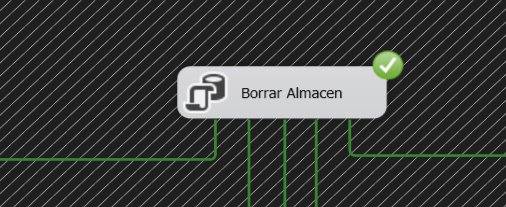
\includegraphics[width=0.65\textwidth]{images/completados/borrado_almacen.png}
			\caption{Carga completa del borrado del almacén}
			\label{fig:borrado_completo}
		\end{center}
	\end{figure}
	
	\subsection{Paciente}
	La primera de las tablas simples son paciente, ya que se extraerá la información directamente de la base de datos y después de una conversión de datos estará listo para ser cargado en el almacén.
	\begin{figure}[H]
		\centering
		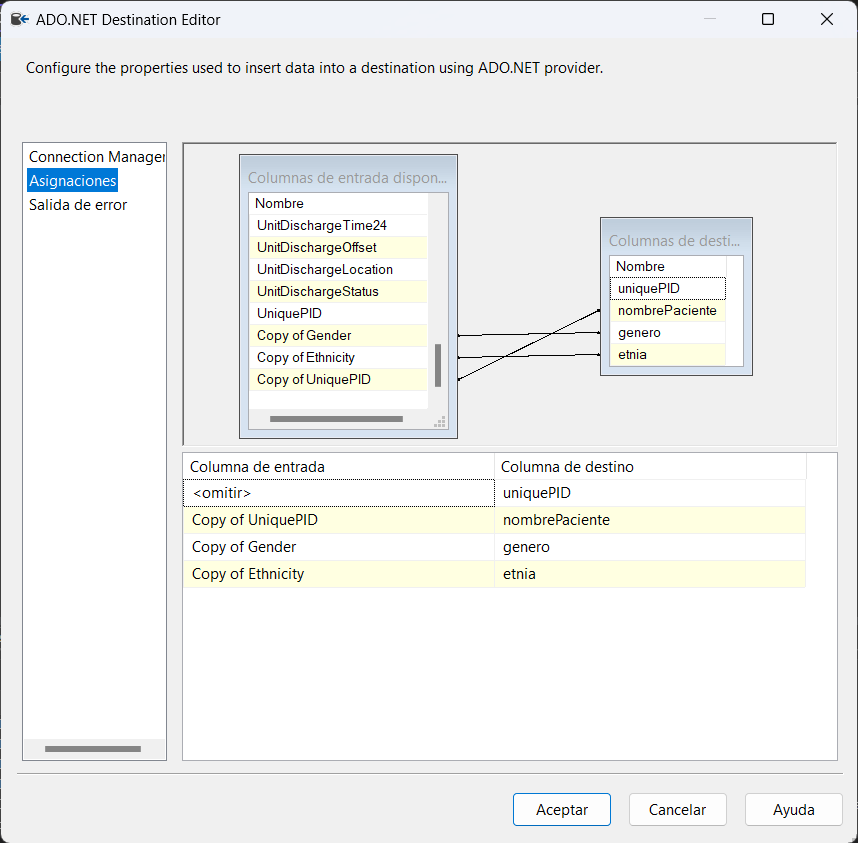
\includegraphics[width=.7\linewidth]{./images/asignaciones/paciente.png}
		\caption{Asignaciones de paciente}
	\end{figure}
	\begin{figure}[H]
		\centering
		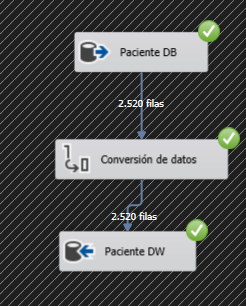
\includegraphics[width=.3\linewidth]{./images/completados/paciente.png}
		\caption{Paciente completado}
	\end{figure}

	\subsection{Medicamento}
	De forma análoga, la tabla medicamento del almacén será cargada solamente con el nombre de droga de la tabla medicamento  de la base de datos y una clave autogenerada.
	\begin{figure}[H]
		\centering
		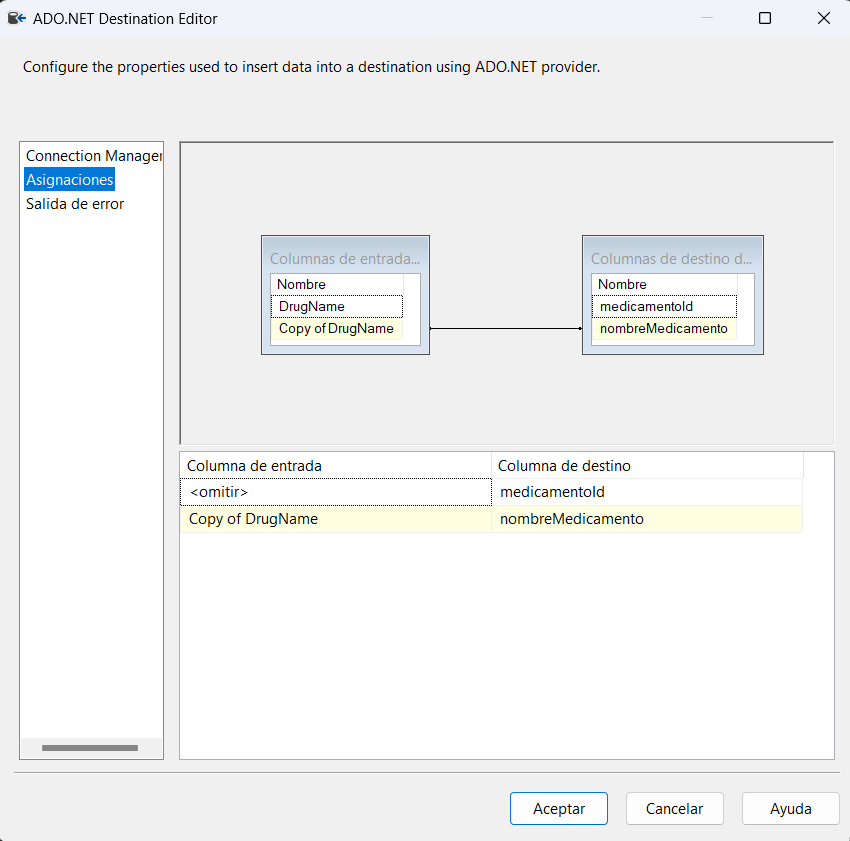
\includegraphics[width=.7\linewidth]{./images/asignaciones/medicamento.png}
		\caption{Asignaciones de medicamento}
	\end{figure}
	
	\begin{figure}[H]
		\centering
		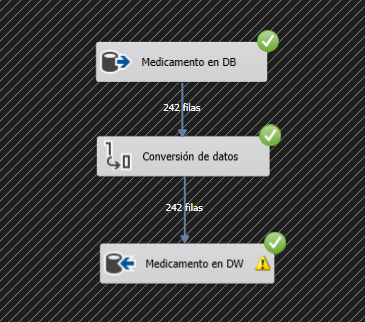
\includegraphics[width=.3\linewidth]{./images/completados/medicamento.png}
		\caption{Medicamento completado}
	\end{figure}

	\subsection{Anyo}
	El año tendrá una clave autogenerada y el atributo anyo será sacado de HospitalDischargeYear de la tabla paciente de la base de datos, indica el año de alta del paciente.
	\begin{figure}[H]
		\centering
		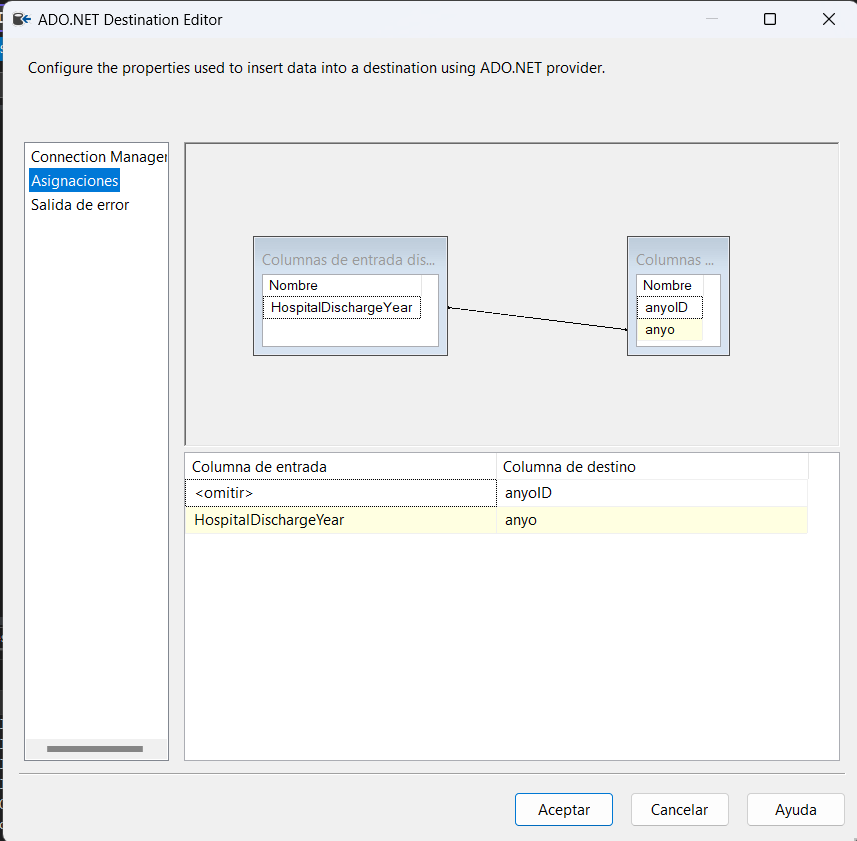
\includegraphics[width=.7\linewidth]{./images/asignaciones/anyo.png}
		\caption{Asignaciones anyo}
	\end{figure}
	\begin{figure}[H]
		\centering
		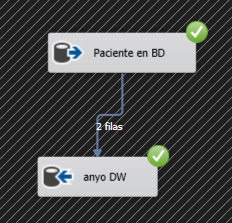
\includegraphics[width=.3\linewidth]{./images/completados/anyo.png}
		\caption{Anyo completado}
	\end{figure}


	\subsection{Estancia Hospital y Ingreso en UCI}
	Continuamos con el proceso de carga de dimensiones jerárquicas de dos niveles. Este procedimiento presenta cierta complejidad debido a la dependencia jerárquica entre los niveles, donde un nivel superior actúa como referencia para el inferior.
	\subsubsection{Estancia Hospital}
	La estancia hospital esta guardado en la tabla paciente de la base de datos, guardamos la fuente de admisión el estado de alta y la clave de la base de datos para poder trazar cada estancia y poder cargar el ingreso en UCI. La clave de esta tabla será autogenerada.
		\begin{figure}[H]
		\centering
		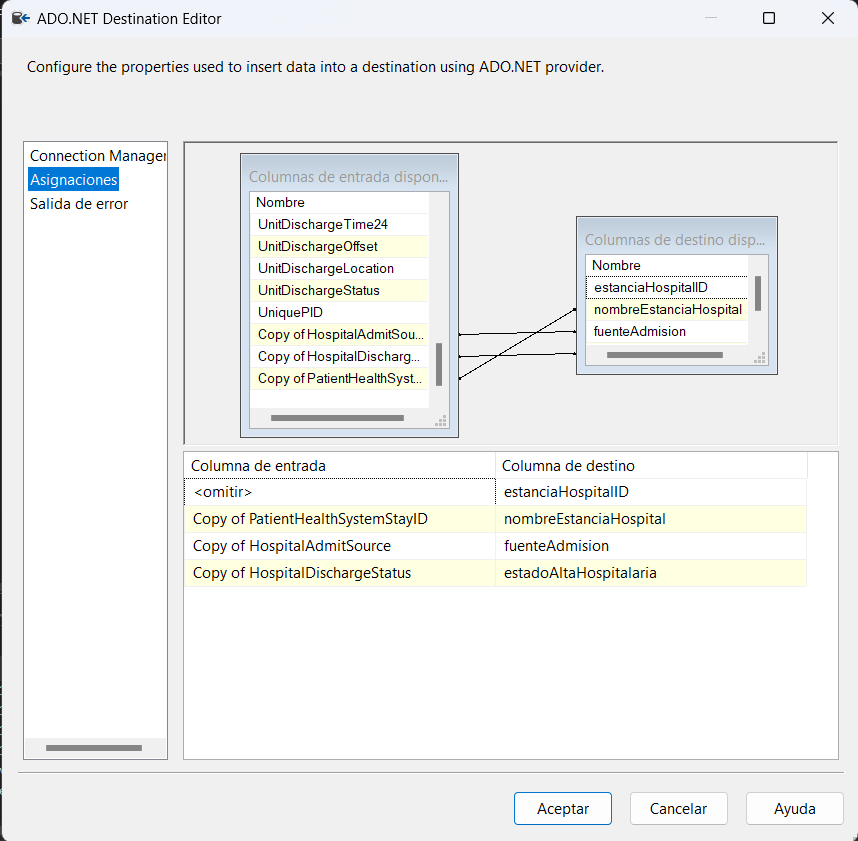
\includegraphics[width=.7\linewidth]{./images/asignaciones/estancia_hospital.png}
		\caption{Asignaciones Estancia Hospital}
	\end{figure}


	\begin{figure}[H]
		\centering
		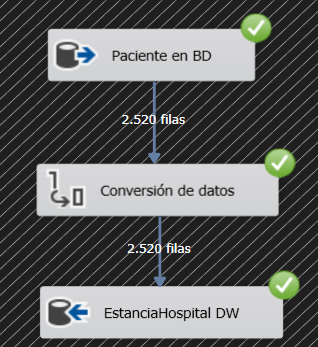
\includegraphics[width=.3\linewidth]{./images/completados/estancia_hospital.png}
		\caption{Completado Estancia hospital}
	\end{figure}
	\subsubsection{Ingreso UCI}
	Como se observa en el flujo de esta tarea, es necesario realizar una búsqueda en nuestro almacén para identificar la clave de la estancia hospitalaria correspondiente a cada ingreso en UCI. Estos datos se encuentran registrados en la tabla paciente, que obtenemos desde la base de datos. 
		\begin{figure}[H]
		\centering
		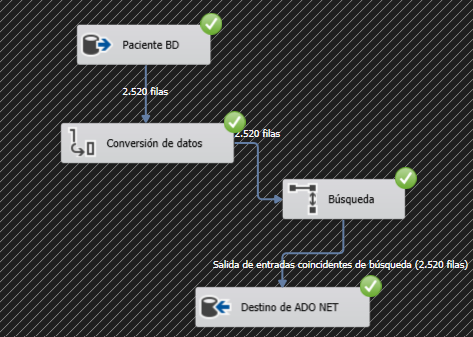
\includegraphics[width=.5\linewidth]{./images/completados/ingreso_uci.png}
		\caption{Completado Ingreso UCI}
	\end{figure}
	\begin{figure}[H]
		\centering
		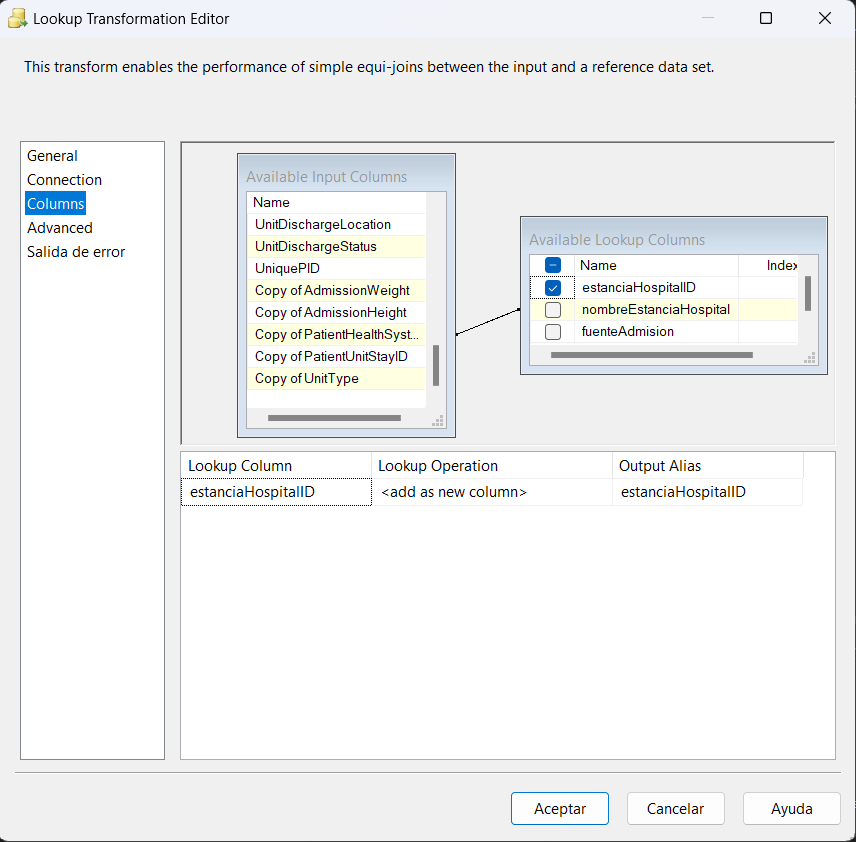
\includegraphics[width=.7\linewidth]{./images/busquedas/ingreso_uci.png}
		\caption{Busqueda ingreso UCI}
	\end{figure}
	Posteriormente, se llevarán a cabo las asignaciones necesarias, tal como se detalla en la Figura \ref{fig:asignaciones_uci}.
	\begin{figure}[H]
		\centering
		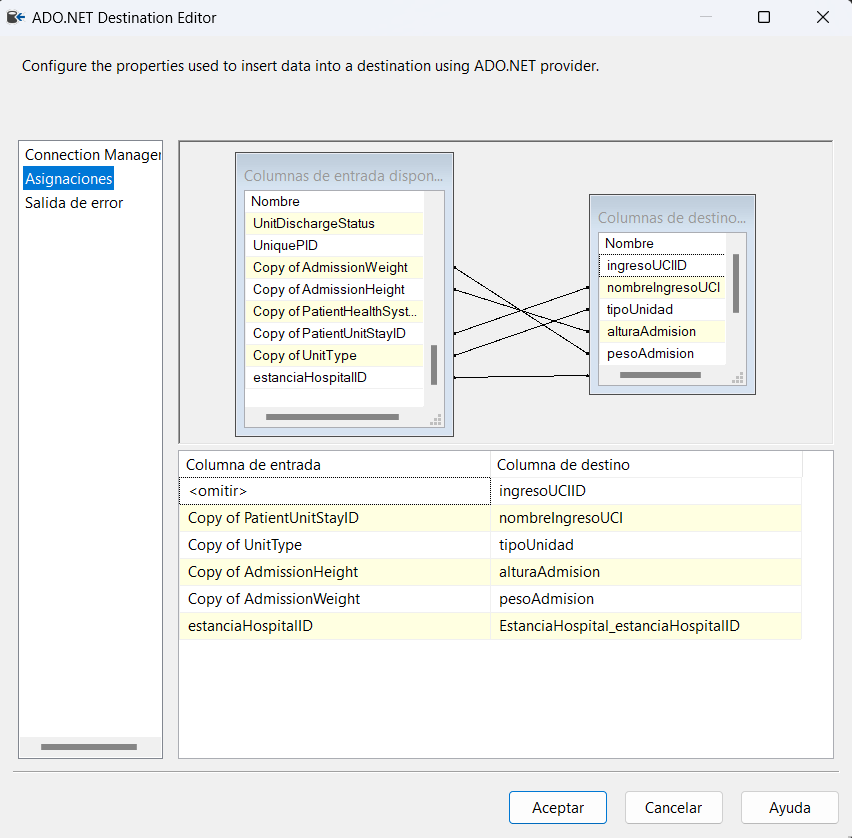
\includegraphics[width=.7\linewidth]{./images/asignaciones/ingreso_uci.png}
		\caption{Asignaciones Ingreso UCI}
		\label{fig:asignaciones_uci}
	\end{figure}

	\subsection{Región y Hospital}
	De forma análoga a la anterior, cargaremos la tabla región y después la tabla hospital
	\subsubsection{Región}
	En esta tabla tendremos una clave autogenerada y el único atributo es el nombre de la región.
	\begin{figure}[H]
		\centering
		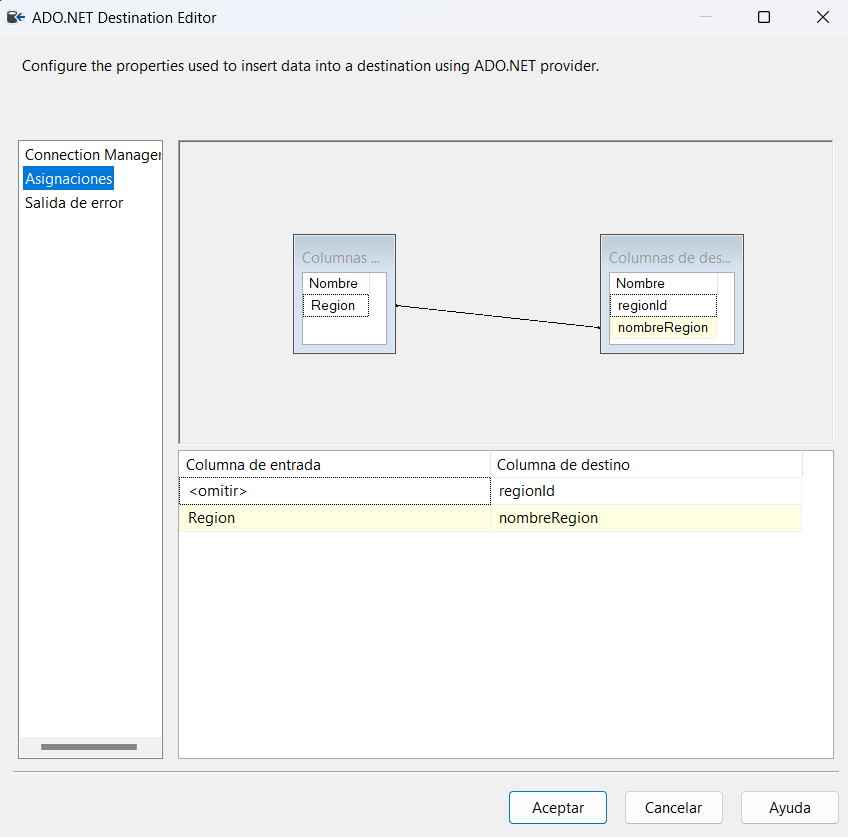
\includegraphics[width=.7\linewidth]{./images/asignaciones/region.png}
		\caption{Asignaciones Región}
	\end{figure}
	\begin{figure}[H]
		\centering
		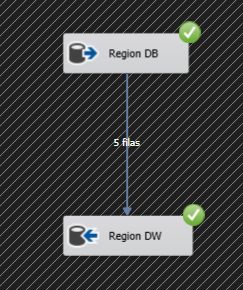
\includegraphics[width=.3\linewidth]{./images/completados/region.png}
		\caption{Completado Región}
	\end{figure}
	\subsubsection{Hospital}
	Esta será la tabla más compleja de toda la carga del almacén de datos debido a las particularidades de los datos, en especial el manejo de hospitales cuyo atributo \textbf{región} es nulo.
	
	El proceso comienza obteniendo todos los hospitales desde la base de datos. Posteriormente, se realiza una \textbf{división condicional} (Figura \ref{fig:division_hospital}) para separar los hospitales en dos grupos: 
	
	\begin{itemize}
		\item \textbf{Hospitales con región:} Para este grupo, se realiza una búsqueda en el almacén de datos con el objetivo de obtener la clave correspondiente a cada región.
		\item \textbf{Hospitales sin región:} Estos registros no requieren la búsqueda de una clave de región, pero deben ser preparados para la integración final.
	\end{itemize}
	
	
	\begin{figure}[H]
		\centering
		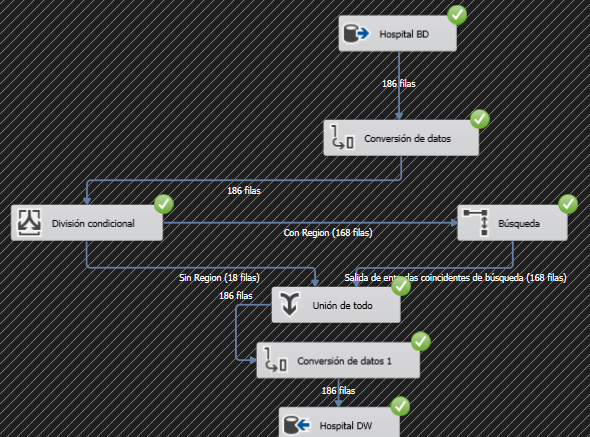
\includegraphics[width=.7\linewidth]{./images/completados/hospital.png}
		\caption{Completado Hospital}
	\end{figure}
	\begin{figure}[H]
		\centering
		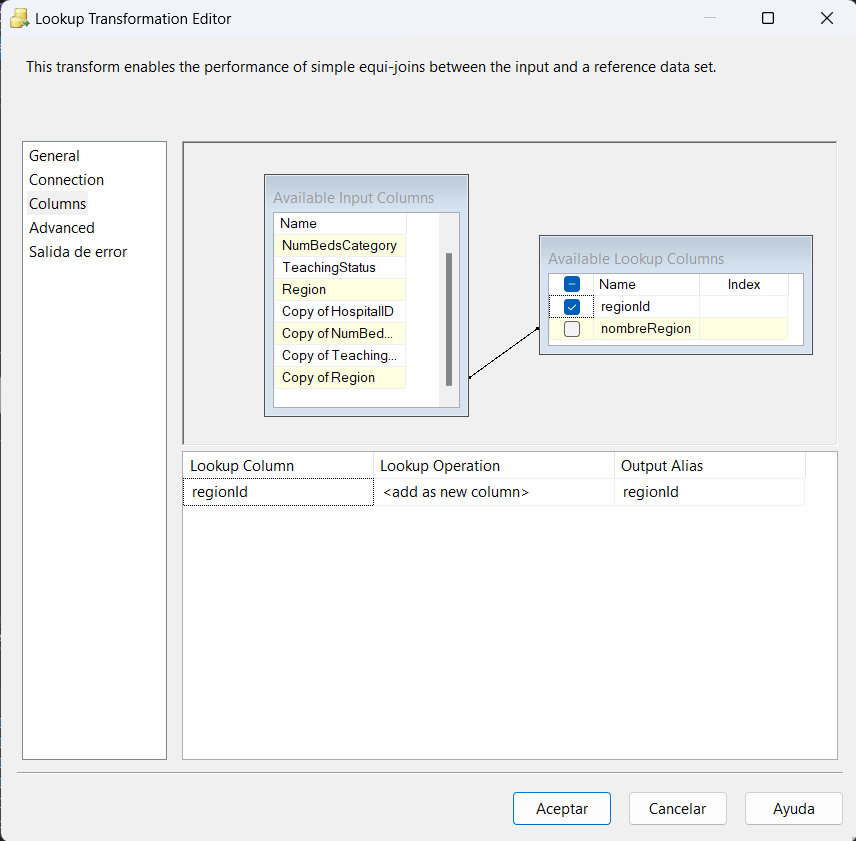
\includegraphics[width=.7\linewidth]{./images/busquedas/hospital_con_region.png}
		\caption{Busqueda de Hospital con región}
	\end{figure}
	\begin{figure}[H]
		\centering
		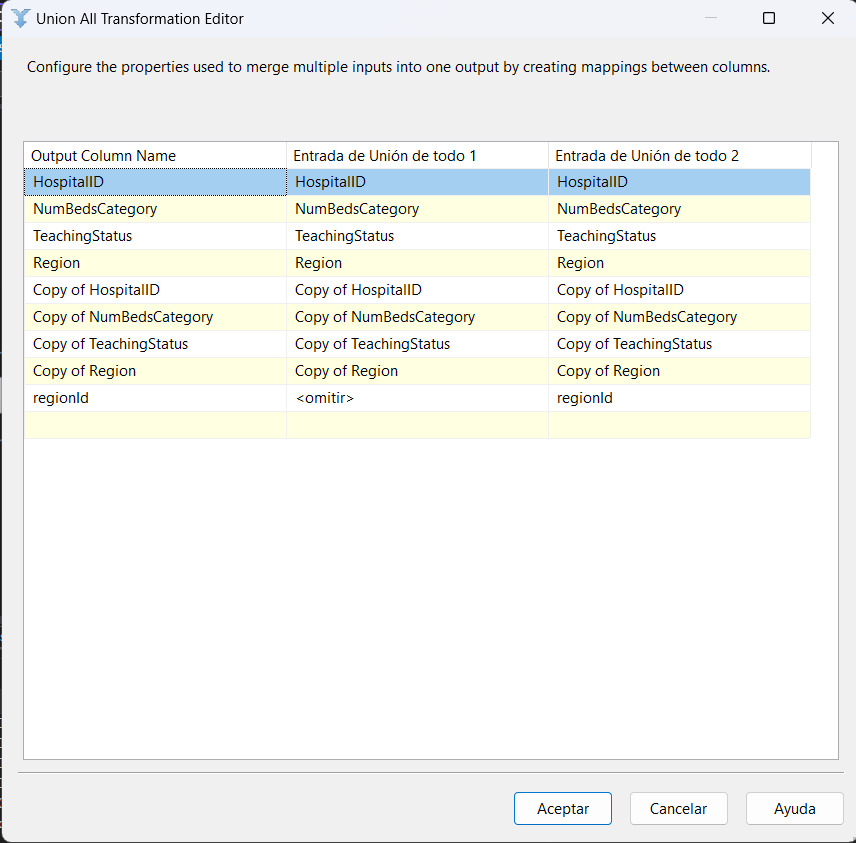
\includegraphics[width=.7\linewidth]{./images/tutorial/union_hospital_con_o_sin_region.png}
		\caption{Busqueda de Hospital sin región}
	\end{figure}
	Finalmente, ambos conjuntos de datos, los hospitales con región (tras realizar la búsqueda) y los hospitales sin región, se \textbf{unen} en una única estructura de datos. Una vez unidos, los datos pasan por una etapa de transformación adicional (\textit{Conversión de datos}) para garantizar su formato correcto antes de cargarlos en la tabla \textit{Hospital} del almacén de datos.

	Este flujo de procesamiento está diseñado para garantizar que todos los registros, independientemente de la disponibilidad del atributo región, se integren correctamente en el almacén de datos. 
	\begin{figure}[H]
		\centering
		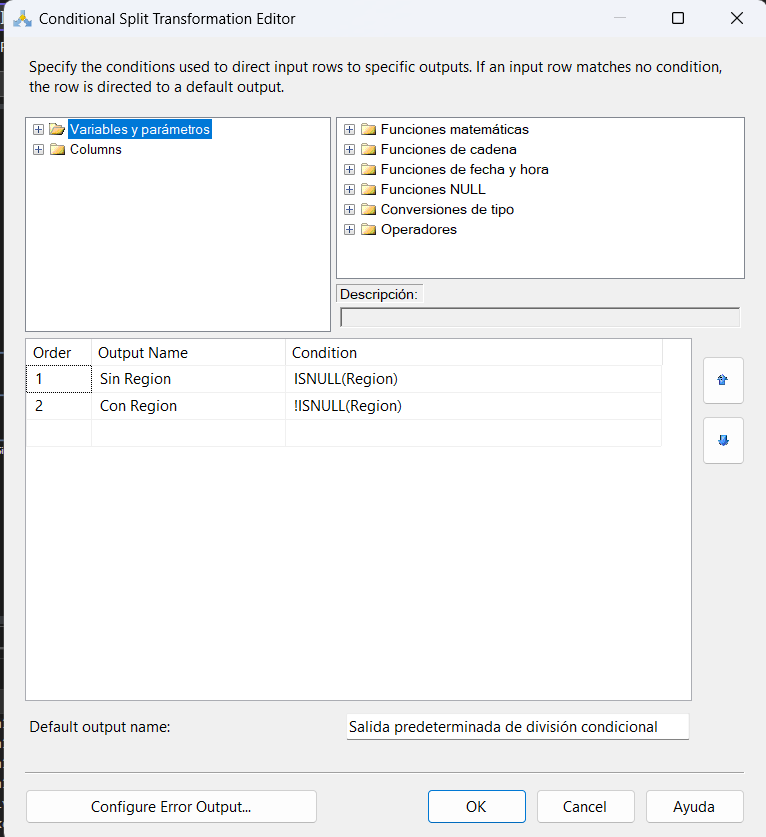
\includegraphics[width=.7\linewidth]{./images/tutorial/division_condicional_hospital_region_null.png}
		\caption{División condicional}
		\label{fig:division_hospital}
	\end{figure}
		\begin{figure}[H]
		\centering
		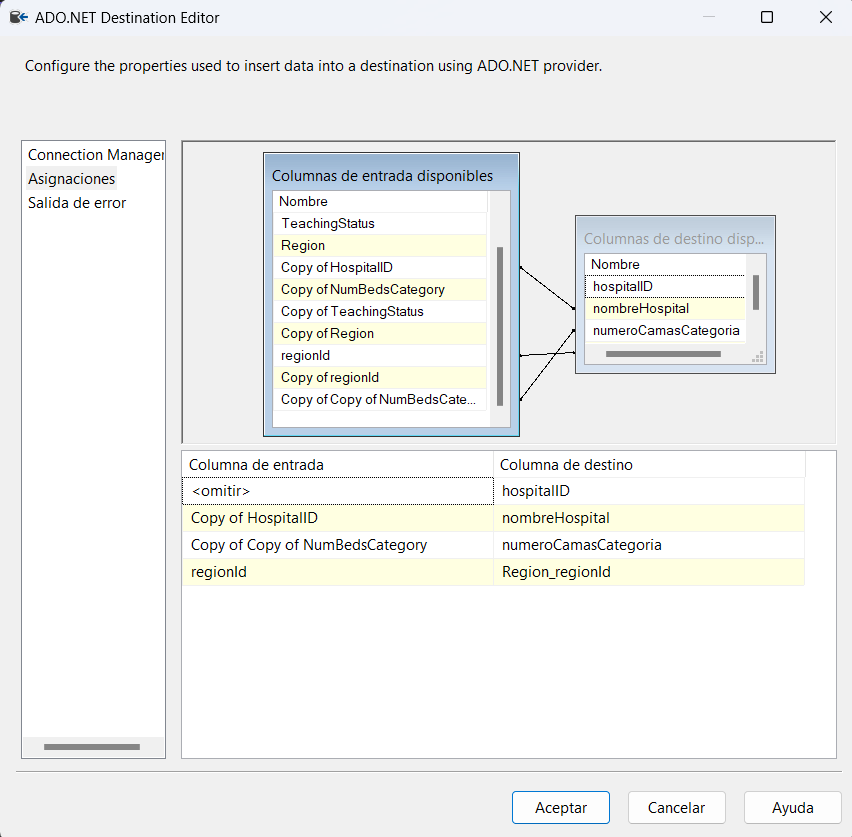
\includegraphics[width=.7\linewidth]{./images/asignaciones/hospital.png}
		\caption{Asignaciones de hospital}
	\end{figure}
	
	\subsection{Gasto Medicamento}
	
	
	Para la carga de la tabla de gasto de medicamentos, se ha construido una consulta SQL que une todas las tablas necesarias mediante relaciones clave y aplica restricciones para filtrar los datos relevantes.
	\\
	
	La consulta selecciona los campos esenciales relacionados con tasas de infusión, volúmenes de fluidos, cantidades de medicamentos, e identificadores únicos de pacientes, años, hospitales, ingresos en UCI y medicamentos. Además, incluye condiciones en el bloque WHERE para garantizar que los registros no tengan valores nulos en los campos clave, asegurando así la calidad de los datos antes de la carga en el almacén (Listing \ref{lst:hecho}).
	\begin{lstlisting}[style=ddlstyle, label=lst:hecho,caption=Consulta para llenado de hecho]
	SELECT 
	infDB.InfusionRate, 
	infDB.VolumeOfFluid, 
	infDB.DrugAmount, 
	paDW.uniquePID, 
	anyDW.anyoID, 
	hospDW.hospitalID, 
	ingrDW.ingresoUCIID, 
	medDW.medicamentoId,
	infDB.InfusionDrugID 
	FROM 
	[eICU Collaborative Research Database].dbo.Patient paDB,
	[eICU Collaborative Research Database].dbo.InfusionDrug infDB,
	UCIDW.dbo.Paciente paDW,
	UCIDW.dbo.Anyo anyDW,
	UCIDW.dbo.Hospital hospDW,
	UCIDW.dbo.IngresoUCI ingrDW,
	UCIDW.dbo.Medicamento medDW
	WHERE 
	paDB.PatientUnitStayID = infDB.PatientUnitStayID 
	AND paDW.nombrePaciente = paDB.UniquePID 
	AND paDB.HospitalDischargeYear = anyDW.anyo 
	AND paDB.HospitalID = hospDW.nombreHospital 
	AND ingrDW.nombreIngresoUCI = paDB.PatientUnitStayID 
	AND infDB.DrugName = medDW.nombreMedicamento 
	AND infDB.InfusionRate IS NOT NULL
	AND infDB.VolumeOfFluid IS NOT NULL
	AND infDB.DrugAmount IS NOT NULL
	AND paDW.uniquePID IS NOT NULL
	AND anyDW.anyoID IS NOT NULL
	AND hospDW.hospitalID IS NOT NULL
	AND ingrDW.ingresoUCIID IS NOT NULL
	AND medDW.medicamentoId IS NOT NULL;
	\end{lstlisting}
	
	
	
	\begin{figure}[H]
		\centering
		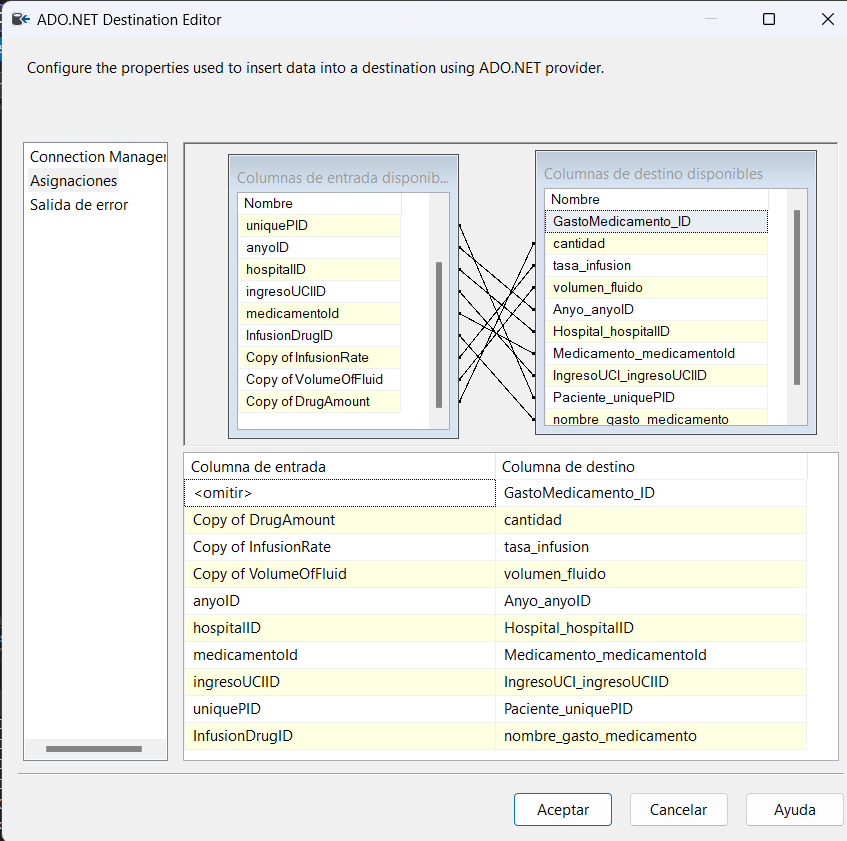
\includegraphics[width=.7\linewidth]{./images/asignaciones/gasto_medicamento.png}
		\caption{Asignaciones gasto medicamento}
	\end{figure}
	\begin{figure}[H]
		\centering
		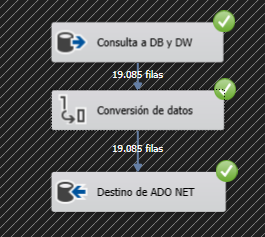
\includegraphics[width=.3\linewidth]{./images/completados/gasto_medicamento.png}
		\caption{Completado gasto en medicamento}
	\end{figure}
	
	Una vez hemos cargado el hecho podemos cargar las relaciones en las que participa el hecho con otra tabla con cardinalidad N:M
	\subsection{Alergia y Relation10}
	Alergia y su tabla intermedia Relation 10 serán cargada de forma secuencial.
	\subsubsection{Alergia}
	La tabla de alergias de la base de datos se mapea de forma sencilla en la tabla correspondiente de nuestro almacén de datos. Sin embargo, solo se conservan los campos relevantes: el nombre de la alergia, el tipo de alergia y, en los casos donde el tipo de alergia corresponde a un medicamento, el nombre de la droga asociada.
	\begin{figure}[H]
		\centering
		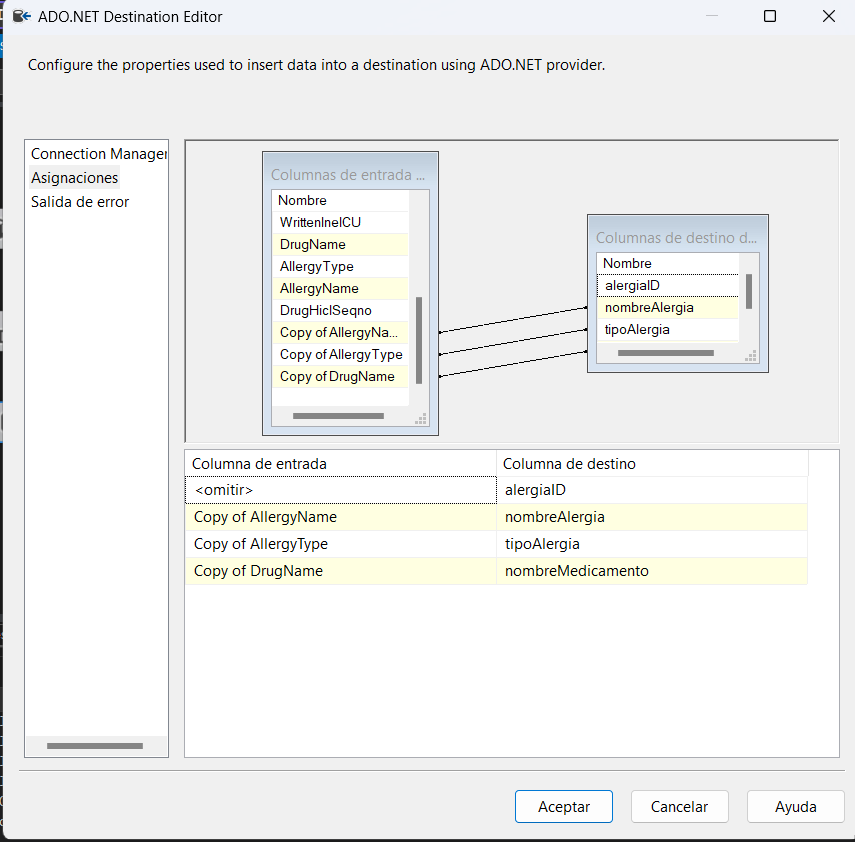
\includegraphics[width=.7\linewidth]{./images/asignaciones/alergia.png}
		\caption{Asignaciones Alergia}
	\end{figure}
	\begin{figure}[H]
		\centering
		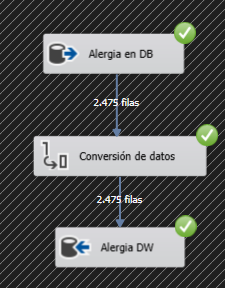
\includegraphics[width=.3\linewidth]{./images/completados/alergia.png}
		\caption{Completado Alergia}
	\end{figure}
	\subsubsection{Relation10}
	
	Para cargar esta tabla también es más claro y sencillo utilizar la consulta Listing \ref{lst:relation10} para cargar las claves de las alergias y del gasto de medicamento del almacén de datos en la tabla intermedia.
	\begin{lstlisting}[style=ddlstyle, label=lst:relation10,caption=Consulta para llenado de relacion 10]
		SELECT DISTINCT
	
	gmDW.GastoMedicamento_ID, allDW.alergiaID
	FROM 
	[eICU Collaborative Research Database].dbo.Patient paDB,
	[eICU Collaborative Research Database].dbo.InfusionDrug infDB,
	[eICU Collaborative Research Database].dbo.Allergy allDB,
	
	UCIDW.dbo.GastoMedicamento gmDW,
	UCIDW.dbo.Alergia allDW
	WHERE 
	paDB.PatientUnitStayID = infDB.PatientUnitStayID  AND 
	paDB.PatientUnitStayID = allDB.PatientUnitStayID   AND
	
	gmDW.nombre_gasto_medicamento = infDB.InfusionDrugID AND
	allDB.AllergyName = allDW.nombreAlergia 
	\end{lstlisting}

	La consulta SQL obtiene combinaciones únicas de \textbf{gasto de medicamentos} y \textbf{alergias} al unir las tablas de la base de datos (\textit{eICU Collaborative Research Database}) y el almacén de datos (\textit{UCIDW}). Se vinculan los registros de medicamentos administrados y las alergias mediante el identificador de estancia del paciente (\texttt{PatientUnitStayID}), y luego se relacionan con los datos de gasto de medicamento y alergia en el almacén. El resultado es una lista de combinaciones únicas entre \textbf{gasto de medicamentos} y \textbf{alergias}.
	
	
	
	
	\begin{figure}[H]
		\centering
		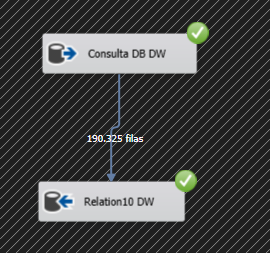
\includegraphics[width=.3\linewidth]{./images/completados/relation10.png}
		\caption{Completado Relation10}
	\end{figure}
	\subsection{Tratamiento y Relation11}
	De manera análoga al anterior se cargará la tabla tratamiento y la relación intermedia entre este y el gasto de medicamento.
	\subsubsection{Tratamiento}
	La carga de la tabla de tratamiento consiste de nuevo en un mapeo directo de los datos desde la base de datos hacia el almacén de datos, conservando únicamente la descripción del tratamiento. Adicionalmente, se incluirá el identificador único de la base de datos para poder identificar cada tratamiento y sus relaciones dentro del almacén, aunque la clave principal en el almacén será autogenerada.
	\begin{figure}[H]
		\centering
		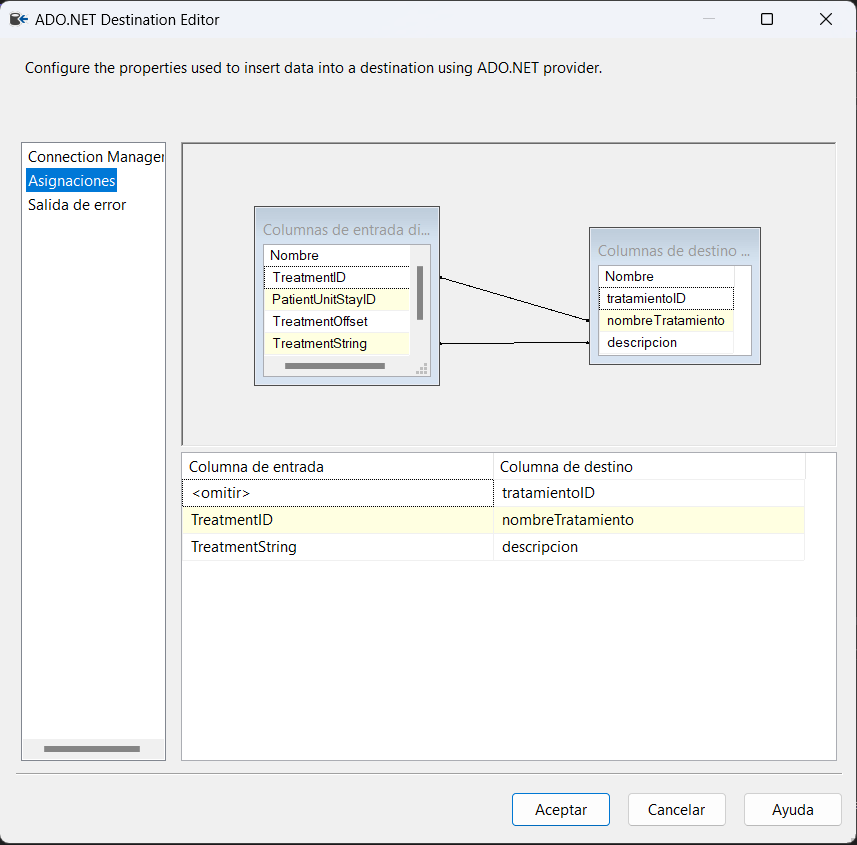
\includegraphics[width=.7\linewidth]{./images/asignaciones/tratamiento.png}
		\caption{Asignación Tratamiento}
	\end{figure}
	\begin{figure}[H]
		\centering
		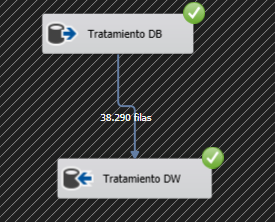
\includegraphics[width=.3\linewidth]{./images/completados/tratamiento.png}
		\caption{Completado Tratamiento}
	\end{figure}
	\subsubsection{Relation11}
	De la misma forma a la relacion 10, será mas sencillo utilizar la consulta Listing \ref{lst:relation11} para quedarnos con las claves de tratamiento y gasto en medicamento de nuestro almacen que estan relacionadas.
	
	\begin{lstlisting}[style=ddlstyle, label=lst:relation11,caption=Consulta para llenado de relacion 11]
	SELECT 
	
	gmDW.GastoMedicamento_ID, trDW.tratamientoID 
	FROM 
	[eICU Collaborative Research Database].dbo.Patient paDB,
	[eICU Collaborative Research Database].dbo.InfusionDrug infDB,
	[eICU Collaborative Research Database].dbo.Treatment trDB,
	
	UCIDW.dbo.GastoMedicamento gmDW,
	UCIDW.dbo.Tratamiento trDW
	WHERE 
	paDB.PatientUnitStayID = infDB.PatientUnitStayID  AND 
	paDB.PatientUnitStayID = trDB.PatientUnitStayID  AND
	
	gmDW.nombre_gasto_medicamento = infDB.InfusionDrugID AND
	trDW.nombreTratamiento = trDB.TreatmentID 
	
	\end{lstlisting}

	La consulta SQL obtiene las combinaciones de \textbf{gasto de medicamentos} y \textbf{tratamientos} al unir las tablas de la base de datos (\textit{eICU Collaborative Research Database}) y el almacén de datos (\textit{UCIDW}). Se relacionan los registros de medicamentos administrados y tratamientos mediante el identificador de estancia del paciente (\texttt{PatientUnitStayID}), y luego se vinculan con los datos correspondientes en el almacén, utilizando los identificadores de gasto de medicamento (\texttt{nombre\_gasto\_medicamento}) y tratamiento (\texttt{nombreTratamiento}). El resultado es una lista de combinaciones entre \textbf{gasto de medicamentos} y \textbf{tratamientos}.
	
	
	\begin{figure}[H]
		\centering
		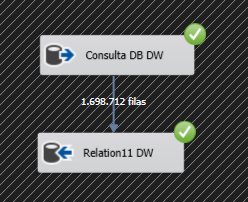
\includegraphics[width=.3\linewidth]{./images/completados/relation11.png}
		\caption{Completado Relation11}
	\end{figure}
		

	\subsection{Dificultades Encontradas}
	\label{sec:dificultades_encontradas}
	
	El principal contratiempo que hemos encontrado ha sido encontrar la forma de que las relaciones de la base de datos fuesen consistentes con las relaciones de el almacén de datos ya que nuestro diseño inicial solo se guardaba una clave autogenerada por tabla del almacén de datos. Para solucionarlo, rediseñamos el almacén como se explicó en la sección anterior con el objetivo de guardar un atributo con el id de la base de datos y que las relaciones sean coherentes. Cabe puntualizar que esto ha sido añadido en las tablas donde sería imposible buscar sin tener ese identificador.
	
	\section{Conclusión}
	\label{sec:conclusion}
	
	Gracias a la correcta implementación del proceso ETL, se ha logrado organizar el almacén de datos de manera eficiente, optimizando la consulta de información relevante para la toma de decisiones. Este proceso ha permitido integrar y transformar datos provenientes de \cite{eicu_crd}. Además, la estructura obtenida no solo asegura la calidad y consistencia de los datos, sino que también sienta las bases para futuras ampliaciones o análisis más complejos, promoviendo la escalabilidad y adaptabilidad del sistema.
	
	En conclusión, este proyecto ETL aporta un modelo sólido y adaptable para la gestión y análisis de datos en el ámbito hospitalario, contribuyendo a una administración más eficiente de los recursos y a una mejora potencial en la atención a los pacientes.
	
	\newpage
	\section{Acceso al Repositorio}
	
	Toda la información adicional, incluyendo el código fuente y la documentación completa de este proyecto, está disponible en el repositorio de GitHub \cite{silva2024github}.
	
	% Incluir la bibliografía
	\bibliographystyle{plain}  % Estilo de la bibliografía (por ejemplo, plain, alpha, ieee, etc.)
	\bibliography{bibli}  % Nombre del archivo .bib sin la extensión
	
\end{document}
